% Options for packages loaded elsewhere
\PassOptionsToPackage{unicode}{hyperref}
\PassOptionsToPackage{hyphens}{url}
%
\documentclass[
  ignorenonframetext,
]{beamer}
\usepackage{pgfpages}
\setbeamertemplate{caption}[numbered]
\setbeamertemplate{caption label separator}{: }
\setbeamercolor{caption name}{fg=normal text.fg}
\beamertemplatenavigationsymbolsempty
% Prevent slide breaks in the middle of a paragraph
\widowpenalties 1 10000
\raggedbottom
\setbeamertemplate{part page}{
  \centering
  \begin{beamercolorbox}[sep=16pt,center]{part title}
    \usebeamerfont{part title}\insertpart\par
  \end{beamercolorbox}
}
\setbeamertemplate{section page}{
  \centering
  \begin{beamercolorbox}[sep=12pt,center]{part title}
    \usebeamerfont{section title}\insertsection\par
  \end{beamercolorbox}
}
\setbeamertemplate{subsection page}{
  \centering
  \begin{beamercolorbox}[sep=8pt,center]{part title}
    \usebeamerfont{subsection title}\insertsubsection\par
  \end{beamercolorbox}
}
\AtBeginPart{
  \frame{\partpage}
}
\AtBeginSection{
  \ifbibliography
  \else
    \frame{\sectionpage}
  \fi
}
\AtBeginSubsection{
  \frame{\subsectionpage}
}
\usepackage{lmodern}
\usepackage{amssymb,amsmath}
\usepackage{ifxetex,ifluatex}
\ifnum 0\ifxetex 1\fi\ifluatex 1\fi=0 % if pdftex
  \usepackage[T1]{fontenc}
  \usepackage[utf8]{inputenc}
  \usepackage{textcomp} % provide euro and other symbols
\else % if luatex or xetex
  \usepackage{unicode-math}
  \defaultfontfeatures{Scale=MatchLowercase}
  \defaultfontfeatures[\rmfamily]{Ligatures=TeX,Scale=1}
\fi
\usetheme[]{Antibes}
\usecolortheme{rose}
% Use upquote if available, for straight quotes in verbatim environments
\IfFileExists{upquote.sty}{\usepackage{upquote}}{}
\IfFileExists{microtype.sty}{% use microtype if available
  \usepackage[]{microtype}
  \UseMicrotypeSet[protrusion]{basicmath} % disable protrusion for tt fonts
}{}
\makeatletter
\@ifundefined{KOMAClassName}{% if non-KOMA class
  \IfFileExists{parskip.sty}{%
    \usepackage{parskip}
  }{% else
    \setlength{\parindent}{0pt}
    \setlength{\parskip}{6pt plus 2pt minus 1pt}}
}{% if KOMA class
  \KOMAoptions{parskip=half}}
\makeatother
\usepackage{xcolor}
\IfFileExists{xurl.sty}{\usepackage{xurl}}{} % add URL line breaks if available
\IfFileExists{bookmark.sty}{\usepackage{bookmark}}{\usepackage{hyperref}}
\hypersetup{
  pdftitle={Primera Revisión del Estatus y Captura Biológicamente Aceptable 2021 para la sardina común de las Regiones de Valparaíso a Los Lagos.},
  pdfauthor={María José Zúñiga},
  hidelinks,
  pdfcreator={LaTeX via pandoc}}
\urlstyle{same} % disable monospaced font for URLs
\newif\ifbibliography
\usepackage{longtable,booktabs}
\usepackage{caption}
% Make caption package work with longtable
\makeatletter
\def\fnum@table{\tablename~\thetable}
\makeatother
\setlength{\emergencystretch}{3em} % prevent overfull lines
\providecommand{\tightlist}{%
  \setlength{\itemsep}{0pt}\setlength{\parskip}{0pt}}
\setcounter{secnumdepth}{-\maxdimen} % remove section numbering

\title{Primera Revisión del Estatus y Captura Biológicamente Aceptable
2021 para la sardina común de las Regiones de Valparaíso a Los Lagos.}
\subtitle{Comité Científico de Pesquerías de Pequeños Pelágicos}
\author{María José Zúñiga}
\date{Sesión N°2: 18-03-2021}
\institute{INSTITUTO DE FOMENTO PESQUERO}

\begin{document}
\frame{\titlepage}

\begin{frame}{Procedimiento de manejo de sardina común}
\protect\hypertarget{procedimiento-de-manejo-de-sardina-comuxfan}{}
\begin{center}
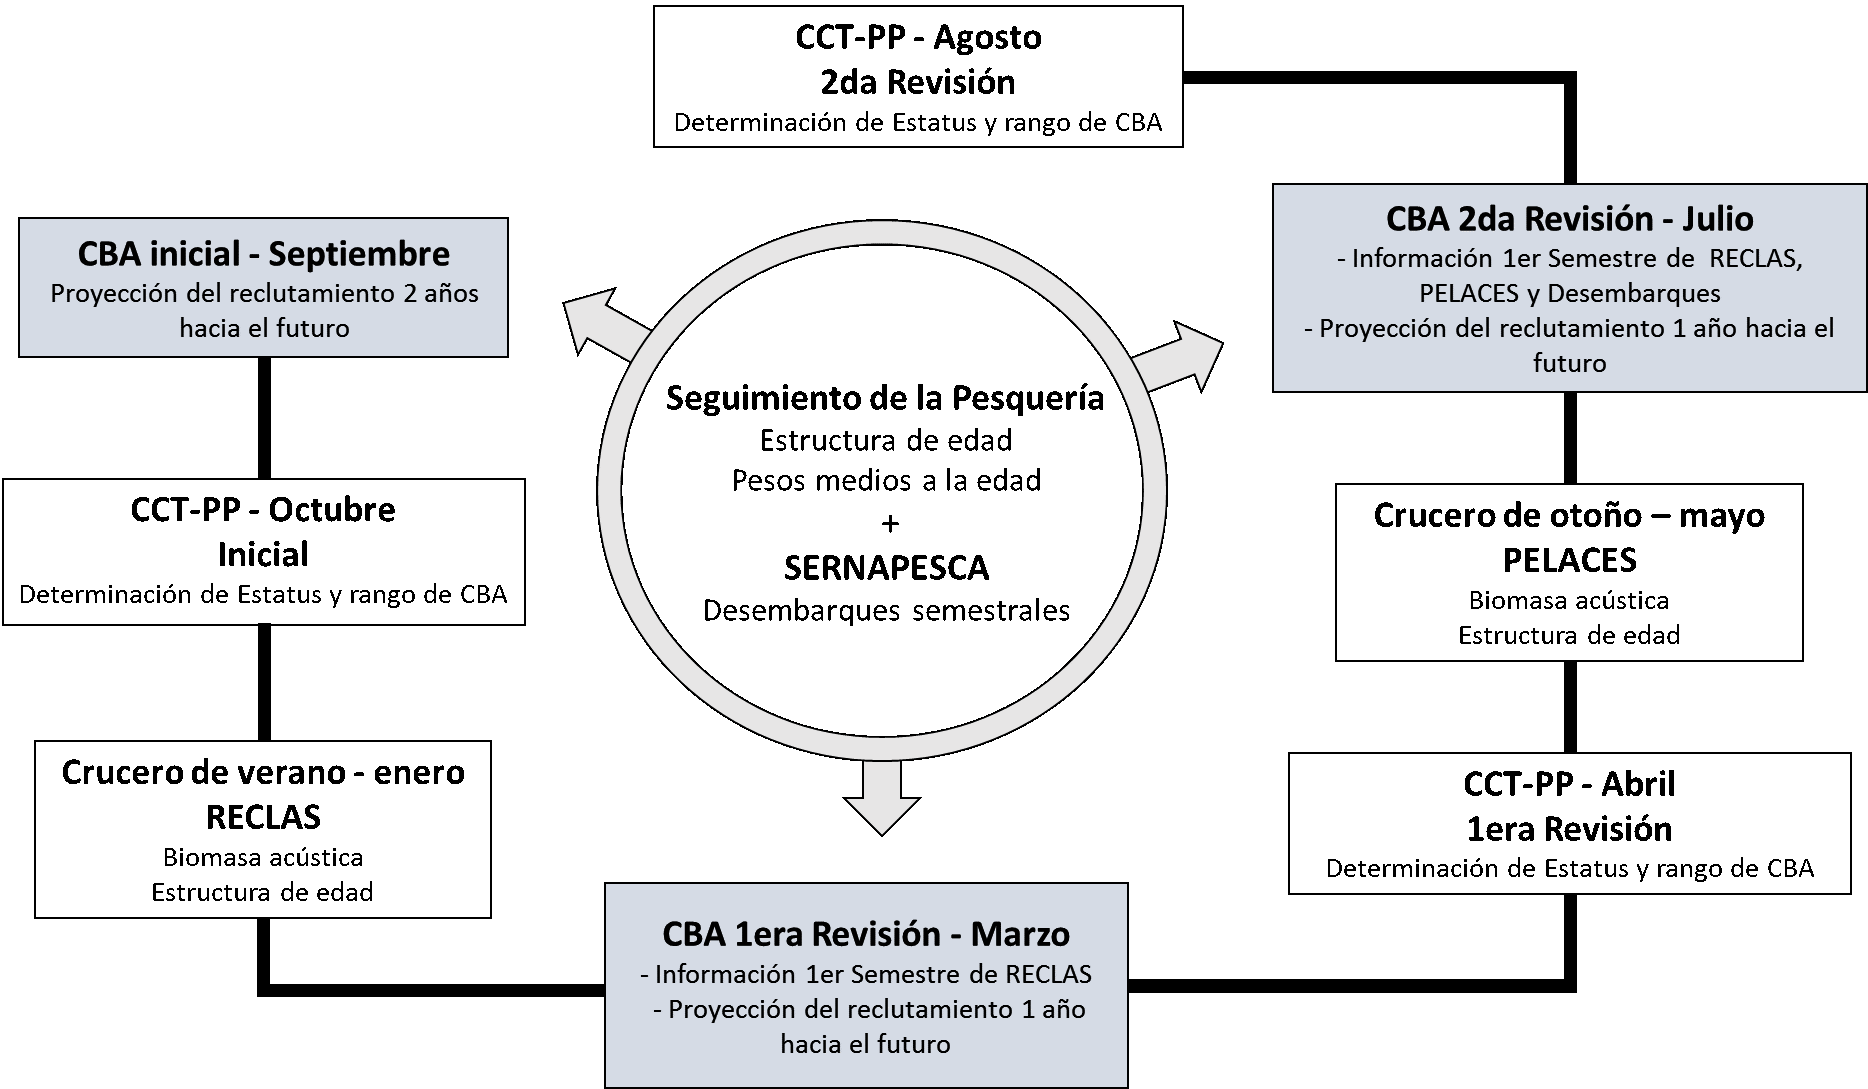
\includegraphics[width=0.9\textwidth]{FigurasInforme_Marzo/Figura14.png}
\end{center}
\end{frame}

\begin{frame}{Datos de entrada de sardina común}
\protect\hypertarget{datos-de-entrada-de-sardina-comuxfan}{}
Datos actualizados

\begin{itemize}
\tightlist
\item
  Biomasa del crucero de verano 2021
\item
  Composición de edad del crucero de verano 2021
\end{itemize}

Datos supuestos

\begin{itemize}
\tightlist
\item
  Captura 2020/21 = desembarque julio-diciembre 2020 +
  70\%CBAinicial2021
\item
  Porcentaje de descarte 2020/21 = 4\%
\item
  Composición de edad de la Flota 2020/2021 = NA
\item
  Pesos medios a la edad Flota 2020/2021 = promedio últimos 5 años
\item
  Biomasa del crucero de otoño 2021 = NA
\item
  Composición de edad del crucero de otoño 2021 = NA
\end{itemize}
\end{frame}

\begin{frame}{Cálculo de Captura 2020/2021 de sardina común}
\protect\hypertarget{cuxe1lculo-de-captura-20202021-de-sardina-comuxfan}{}
\begin{itemize}
\item
  Desembarque 2do semestre 2020 = 69.841 toneladas
\item
  Captura 2021 = 0,7xCBAinicial = 140.986 toneladas
\item
  Captura 2020/21 sin incorporar el descarte = 210.827 toneladas
\item
  \% de descarte 2020/21 = 4\% = 8.433 toneladas
\item
  Captura 2020/21 + 4\%descarte 2020/21 = 219.260 toneladas
\end{itemize}
\end{frame}

\begin{frame}{Ajustes del modelo a los datos - sardina común}
\protect\hypertarget{ajustes-del-modelo-a-los-datos---sardina-comuxfan}{}
\begin{center}
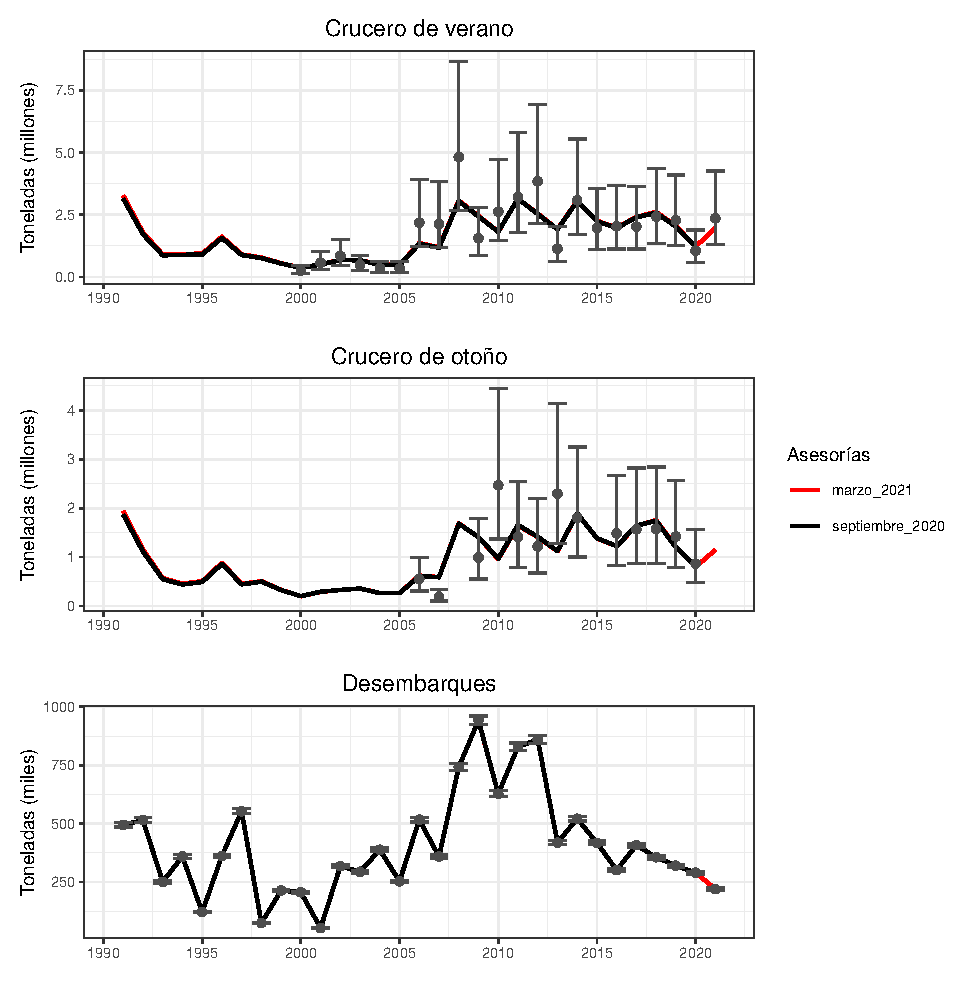
\includegraphics[width=0.7\textwidth]{FigurasInforme_Marzo/Fig26_Ajustes_indices-1.pdf}
\end{center}
\end{frame}

\begin{frame}{Ajuste Flota de sardina común}
\protect\hypertarget{ajuste-flota-de-sardina-comuxfan}{}
\begin{center}

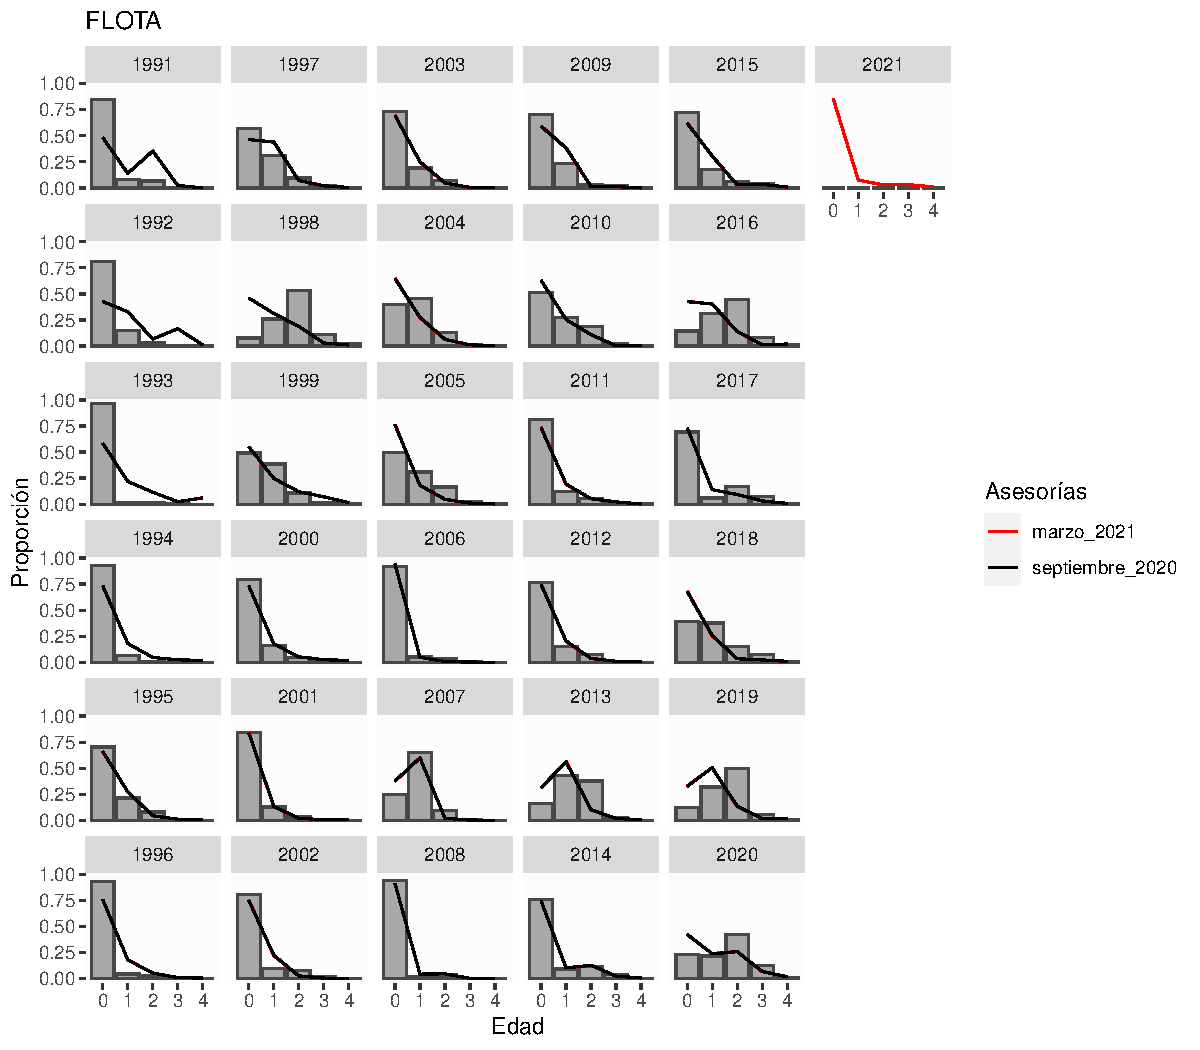
\includegraphics[width=0.8\textwidth]{FigurasInforme_Marzo/Fig28_ajustesCompF-1.pdf}

\end{center}
\end{frame}

\begin{frame}{Ajuste Crucero de verano de sardina común}
\protect\hypertarget{ajuste-crucero-de-verano-de-sardina-comuxfan}{}
\begin{center}

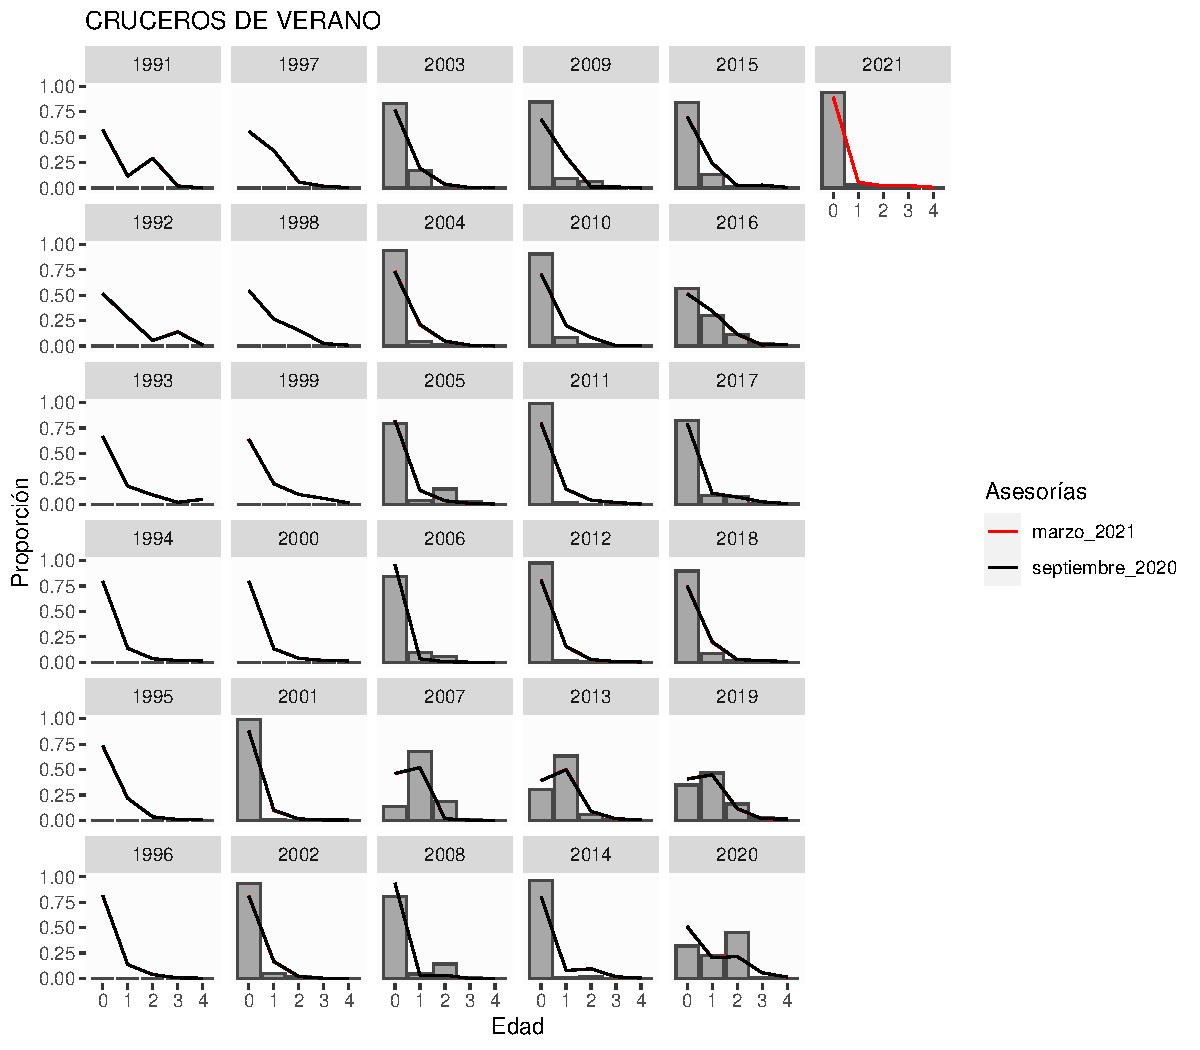
\includegraphics[width=0.8\textwidth]{FigurasInforme_Marzo/Fig29_ajustesCompR-1.pdf}

\end{center}
\end{frame}

\begin{frame}{Ajuste Crucero de otoño de sardina común}
\protect\hypertarget{ajuste-crucero-de-otouxf1o-de-sardina-comuxfan}{}
\begin{center}

\includegraphics[width=0.8\textwidth]{FigurasInforme_Marzo/Fig30_AjustesCompP-1.pdf}

\end{center}
\end{frame}

\begin{frame}{Indicadores poblacionales de sardina común}
\protect\hypertarget{indicadores-poblacionales-de-sardina-comuxfan}{}
\begin{center}
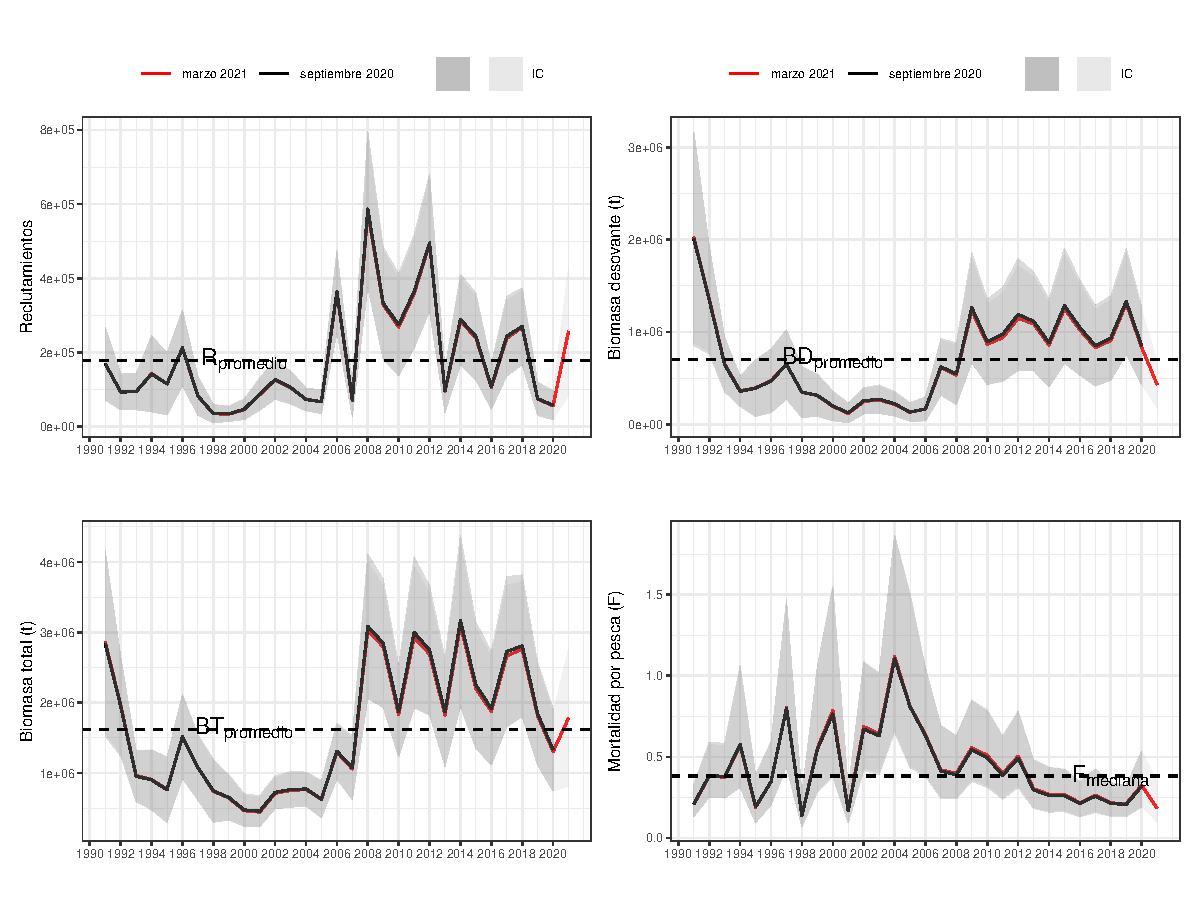
\includegraphics[width=0.9\textwidth]{FigurasInforme_Marzo/F35_Varpobl-1.pdf}
\end{center}
\end{frame}

\begin{frame}{Puntos Biológicos de Referencia de sardina común}
\protect\hypertarget{puntos-bioluxf3gicos-de-referencia-de-sardina-comuxfan}{}
\begin{block}{BD\textasciitilde0\textasciitilde,
BD\textasciitilde RMS\textasciitilde,
BD\textasciitilde LIM\textasciitilde{} y
F\textasciitilde RMS\textasciitilde{}}
\protect\hypertarget{bd0-bdrms-bdlim-y-frms}{}
\begin{center}
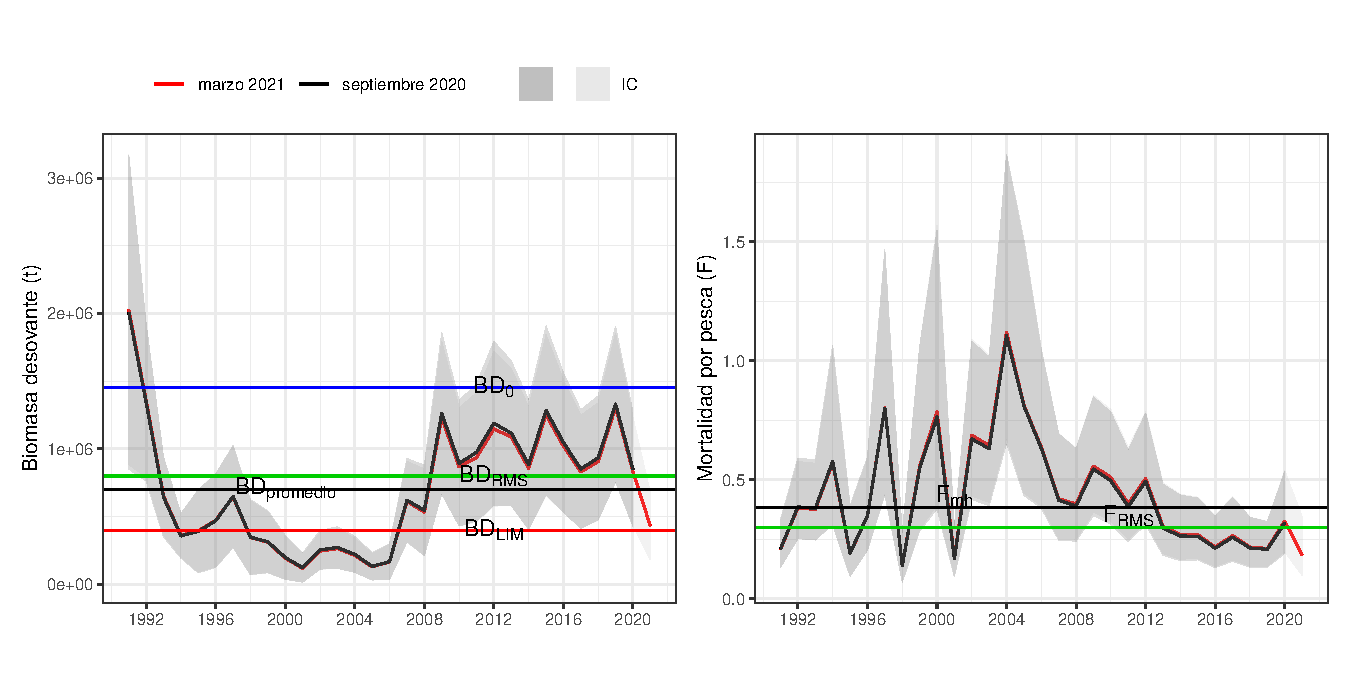
\includegraphics[width=0.99\textwidth]{FigurasInforme_Marzo/F37_PBRs_Bmed_Fmed-1.pdf}
\end{center}
\end{block}
\end{frame}

\begin{frame}{Indicadores del estado de sardina común}
\protect\hypertarget{indicadores-del-estado-de-sardina-comuxfan}{}
\begin{center}
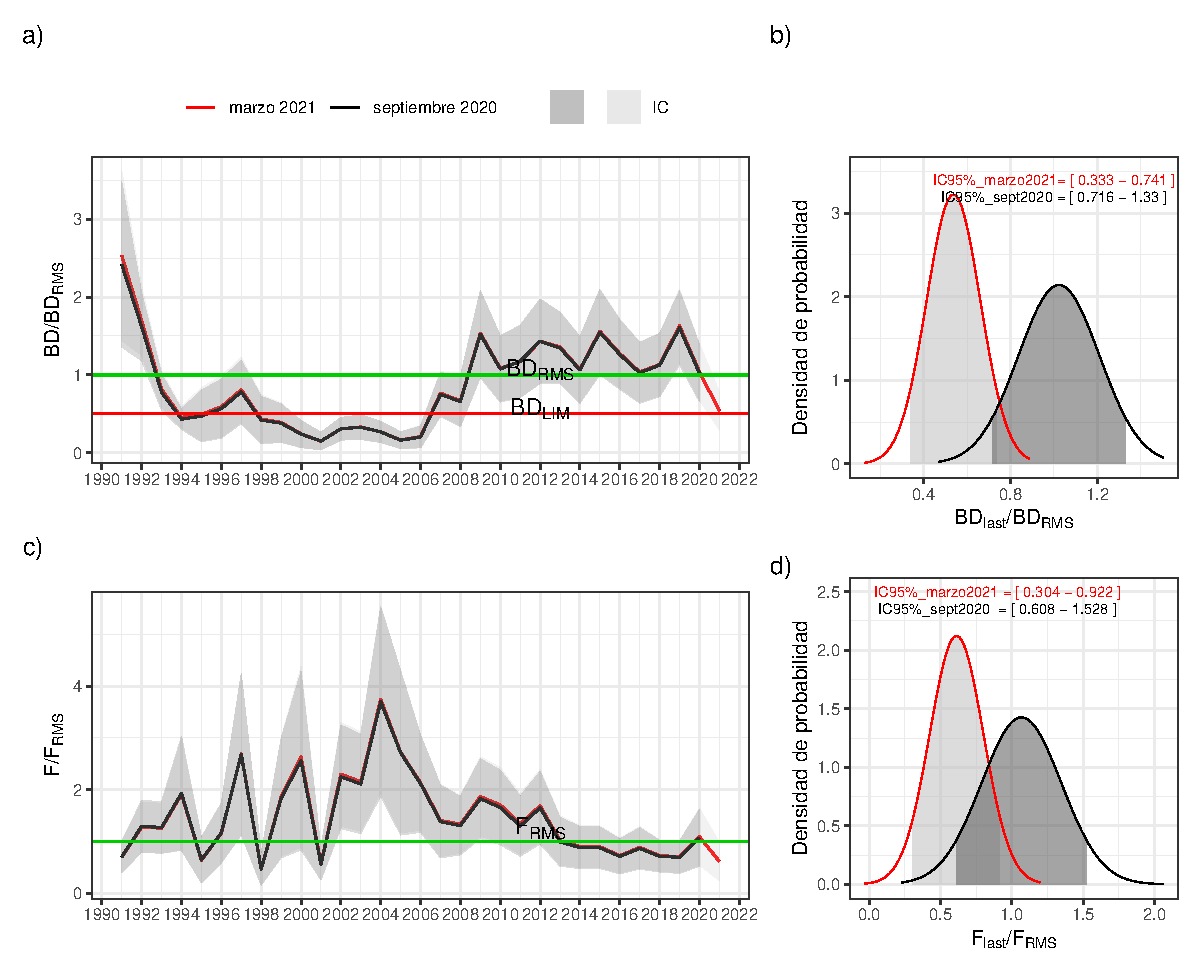
\includegraphics[width=0.9\textwidth]{FigurasInforme_Marzo/F39_indicadoresStock-1.pdf}
\end{center}
\end{frame}

\begin{frame}{Estatus 2019/20 de sardina común}
\protect\hypertarget{estatus-201920-de-sardina-comuxfan}{}
\begin{center}
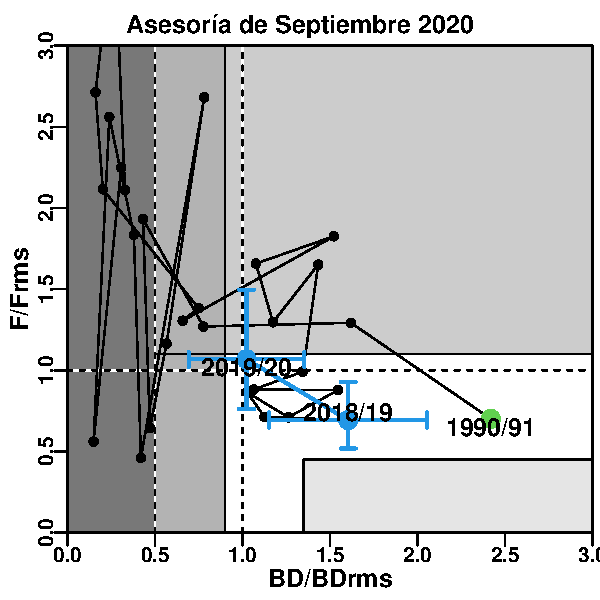
\includegraphics[width=0.65\textwidth]{FigurasInforme_Marzo/Fig40_DFsept-1.pdf}
\end{center}
\end{frame}

\begin{frame}{Estatus 2020/21 de sardina común}
\protect\hypertarget{estatus-202021-de-sardina-comuxfan}{}
\begin{center}
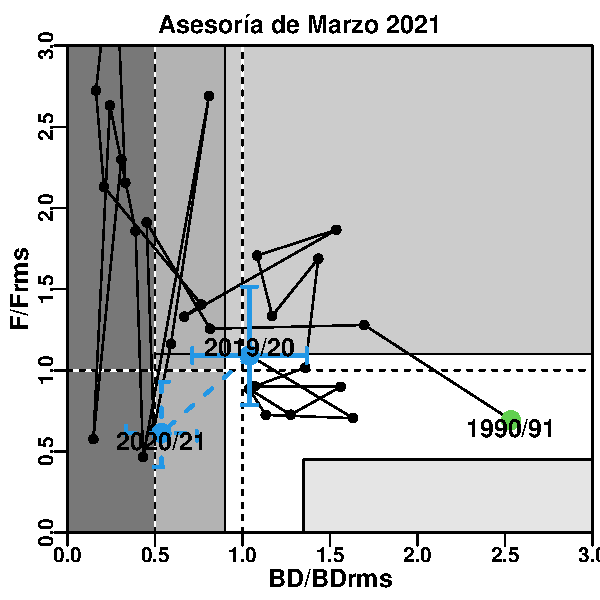
\includegraphics[width=0.65\textwidth]{FigurasInforme_Marzo/Fig41_DFmarzo-1.pdf}
\end{center}
\end{frame}

\begin{frame}{Estatus proyectado año biológico 2020/21 y 2021/22 de
sardina común}
\protect\hypertarget{estatus-proyectado-auxf1o-bioluxf3gico-202021-y-202122-de-sardina-comuxfan}{}
\begin{columns}
\column{0.5\textwidth}
\begin{center} 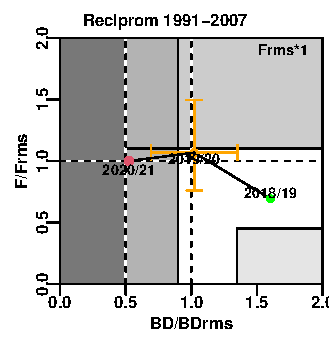
\includegraphics[width=0.9\textwidth]{FigurasInforme_Marzo/Fig44a_sept-1.pdf}\end{center}
\column{0.5\textwidth}
\begin{center} 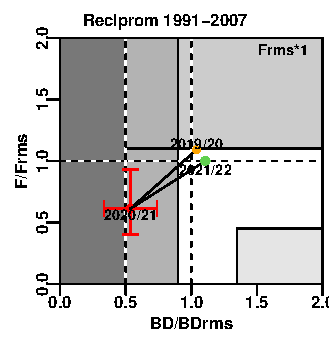
\includegraphics[width=0.9\textwidth]{FigurasInforme_Marzo/Fig45a_marzo-1.pdf}\end{center}
\end{columns}

\footnotesize

\begin{itemize}
\item
  100\% de probabilidad de sobre-explotación y 42\% de probabilidad de
  colapso para el año \textbf{2020/2021}
\item
  27\% de probabilidad de sobre-explotación y 4\% de probabilidad de
  colapso para el año \textbf{2021/2022}
\end{itemize}
\end{frame}

\begin{frame}{Incertidumbre del Estatus 2019/20 y 2020/21 de sardina
común}
\protect\hypertarget{incertidumbre-del-estatus-201920-y-202021-de-sardina-comuxfan}{}
\begin{table}
    \centering
    \resizebox{10cm}{!} {
    \begin{tabular}{|l|c|c|c|c|c|}
    \hline
                            & Sept 2020 & Marzo 2021 \\
                            & $Estatus_{2019/20}$ & $Estatus_{2020/21}$ \\ \hline
   $BD_{last}<BD_{RMS}$     &   0,45    & 1,00 \\
   $F_{last}>F_{RMS}$       &   0,60    & 0,02 \\ \hline
   Sobre-explotación        &   0,26    & 1,00 \\
   Agotamiento/colapso      &   0,00    & 0,38 \\
   Sobrepesca               &   0,45    & 0,00 \\ \hline
    \end{tabular}}
    \end{table}
\end{frame}

\begin{frame}{Supuestos de proyección de sardina común}
\protect\hypertarget{supuestos-de-proyecciuxf3n-de-sardina-comuxfan}{}
\small
Se proyecta dos años biológicos hacia el futuro bajo los siguientes supuestos:

-   Escenarios de Reclutamiento promedio:

    * Promedio período favorable: años 2008-2012
    
    * Promedio período reciente: años 2013-2021
    
    * Promedio período desfavorable: años 1991-2007

-   Pesos medios igual al promedio de los últimos 5 años

-   Mortalidad por pesca igual a $F_{RMS}$

-   Proporción semestral de captura 70\% primer semestre y 30\% segundo semestre

-   supuesto de descarte 4%
\end{frame}

\begin{frame}{Proporción semestral de las capturas de sardina común}
\protect\hypertarget{proporciuxf3n-semestral-de-las-capturas-de-sardina-comuxfan}{}
$CBA_{2021} = 70\%CBA_{2020/21} + 30\%CBA_{2021/22}$

\begin{center}

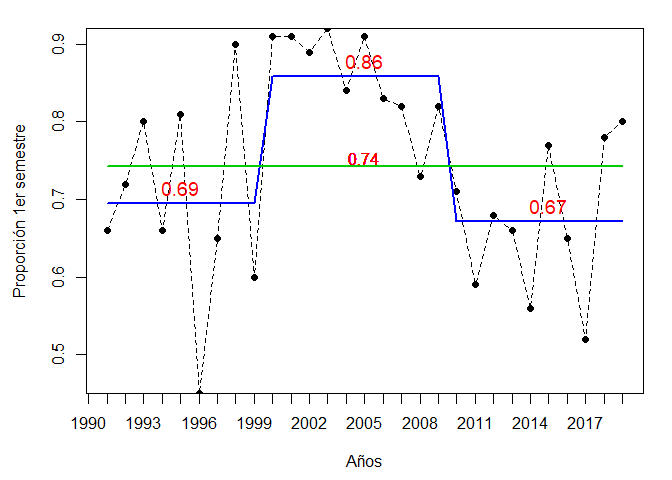
\includegraphics[width=0.7\textwidth]{FigurasInforme_Marzo/Fig17_metod_cbaprop.png}

\end{center}
\end{frame}

\begin{frame}{Reclutamientos promedios proyectados - sardina común}
\protect\hypertarget{reclutamientos-promedios-proyectados---sardina-comuxfan}{}
\begin{center}
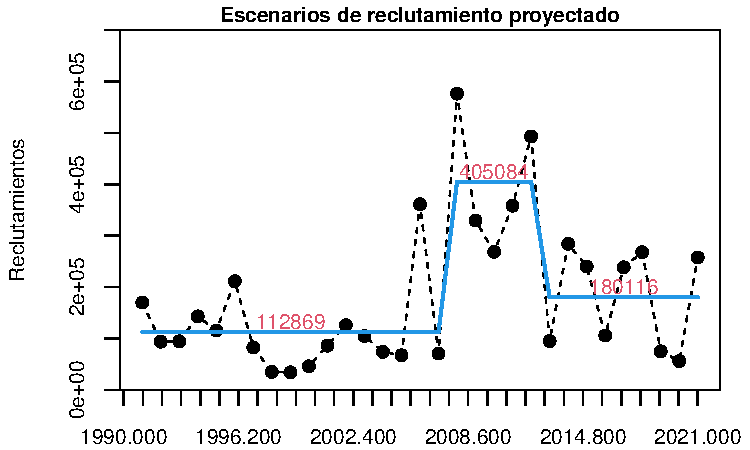
\includegraphics[width=0.9\textwidth]{FigurasInforme_Marzo/Fig43_Reclproy_marzo-1.pdf}
\end{center}
\end{frame}

\begin{frame}{Rango de la Primera revisión de la CBA 2021 de sardina
común}
\protect\hypertarget{rango-de-la-primera-revisiuxf3n-de-la-cba-2021-de-sardina-comuxfan}{}
\begin{block}{CBA}
\protect\hypertarget{cba}{}
\begin{table}
    \centering
    \resizebox{7cm}{!} {
    \begin{tabular}{|c|c|c|c|}
    \hline
    &\multicolumn{3}{|c|}{Escenarios de Reclutamiento} \\ 
      Percentil de Crms & 1991-2007 & 2008-2012 & 2013-2020\\ \hline
      10\%              & 234.063   & 269.084    & 236.111\\ 
      20\%              & 246.990   & 284.170    & 251.030\\ 
      30\%              & 256.311   & 295.048    & 261.787\\ 
      40\%              & 264.276   & 304.342    & 270.979\\ 
      50\%              & 271.720   & 313.030    & 279.570\\ \hline
    \end{tabular}}
    \end{table}
\end{block}

\begin{block}{Resguardo de la Captura al RMS}
\protect\hypertarget{resguardo-de-la-captura-al-rms}{}
\begin{table}
    \centering
    \resizebox{7cm}{!} {
    \begin{tabular}{|c|c|c|c|}
    \hline
    &\multicolumn{3}{|c|}{Escenarios de Reclutamiento} \\ 
      Percentil de Crms & 1991-2007 & 2008-2012 &  2013-2020\\ \hline
     10\%               & 0.14     & 0.14      & 0.16 \\ 
     20\%               & 0.09      & 0.09      & 0.10  \\ 
     30\%               & 0.06      & 0.06      & 0.06 \\ 
     40\%               & 0.03      & 0.03      & 0.03 \\ 
     50\%               & 0         & 0         &  0 \\ \hline
    \end{tabular}}
        \end{table}
\end{block}
\end{frame}

\begin{frame}{Descuento del 4\% descarte - sardina común}
\protect\hypertarget{descuento-del-4-descarte---sardina-comuxfan}{}
\begin{longtable}[]{@{}cccc@{}}
\toprule
\begin{minipage}[b]{0.19\columnwidth}\centering
Percentil de C\textsubscript{RMS}\strut
\end{minipage} & \begin{minipage}[b]{0.23\columnwidth}\centering
Reclutamiento 1991-2007\strut
\end{minipage} & \begin{minipage}[b]{0.23\columnwidth}\centering
Reclutamiento 2008-2012\strut
\end{minipage} & \begin{minipage}[b]{0.23\columnwidth}\centering
Reclutamiento 2013-2020\strut
\end{minipage}\tabularnewline
\midrule
\endhead
\begin{minipage}[t]{0.19\columnwidth}\centering
10\%\strut
\end{minipage} & \begin{minipage}[t]{0.23\columnwidth}\centering
224.700\strut
\end{minipage} & \begin{minipage}[t]{0.23\columnwidth}\centering
258.321\strut
\end{minipage} & \begin{minipage}[t]{0.23\columnwidth}\centering
226.667\strut
\end{minipage}\tabularnewline
\begin{minipage}[t]{0.19\columnwidth}\centering
20\%\strut
\end{minipage} & \begin{minipage}[t]{0.23\columnwidth}\centering
237.110\strut
\end{minipage} & \begin{minipage}[t]{0.23\columnwidth}\centering
272.803\strut
\end{minipage} & \begin{minipage}[t]{0.23\columnwidth}\centering
240.989\strut
\end{minipage}\tabularnewline
\begin{minipage}[t]{0.19\columnwidth}\centering
30\%\strut
\end{minipage} & \begin{minipage}[t]{0.23\columnwidth}\centering
246.059\strut
\end{minipage} & \begin{minipage}[t]{0.23\columnwidth}\centering
283.246\strut
\end{minipage} & \begin{minipage}[t]{0.23\columnwidth}\centering
251.316\strut
\end{minipage}\tabularnewline
\begin{minipage}[t]{0.19\columnwidth}\centering
40\%\strut
\end{minipage} & \begin{minipage}[t]{0.23\columnwidth}\centering
253.705\strut
\end{minipage} & \begin{minipage}[t]{0.23\columnwidth}\centering
292.169\strut
\end{minipage} & \begin{minipage}[t]{0.23\columnwidth}\centering
260.140\strut
\end{minipage}\tabularnewline
\begin{minipage}[t]{0.19\columnwidth}\centering
50\%\strut
\end{minipage} & \begin{minipage}[t]{0.23\columnwidth}\centering
260.851\strut
\end{minipage} & \begin{minipage}[t]{0.23\columnwidth}\centering
300.509\strut
\end{minipage} & \begin{minipage}[t]{0.23\columnwidth}\centering
268.387\strut
\end{minipage}\tabularnewline
\bottomrule
\end{longtable}

CBA inicial 2021 = 201.409 toneladas (percentil del 20\%, escenario de
reclutamiento bajo período 1991-2007 y 6\% de descarte)
\end{frame}

\begin{frame}{Diferencia porcentual entre CBA inicial - 6\%descarte y
Primera revisión de CBA - 4\% descarte}
\protect\hypertarget{diferencia-porcentual-entre-cba-inicial---6descarte-y-primera-revisiuxf3n-de-cba---4-descarte}{}
diferencia = 1-(1erarevisiónCBA/CBAinicial)*100

\begin{longtable}[]{@{}cccc@{}}
\toprule
\begin{minipage}[b]{0.19\columnwidth}\centering
Percentil de C\textsubscript{RMS}\strut
\end{minipage} & \begin{minipage}[b]{0.23\columnwidth}\centering
Reclutamiento 1991-2007\strut
\end{minipage} & \begin{minipage}[b]{0.23\columnwidth}\centering
Reclutamiento 2008-2012\strut
\end{minipage} & \begin{minipage}[b]{0.23\columnwidth}\centering
Reclutamiento 2013-2020\strut
\end{minipage}\tabularnewline
\midrule
\endhead
\begin{minipage}[t]{0.19\columnwidth}\centering
10\%\strut
\end{minipage} & \begin{minipage}[t]{0.23\columnwidth}\centering
22\strut
\end{minipage} & \begin{minipage}[t]{0.23\columnwidth}\centering
-22\strut
\end{minipage} & \begin{minipage}[t]{0.23\columnwidth}\centering
8\strut
\end{minipage}\tabularnewline
\begin{minipage}[t]{0.19\columnwidth}\centering
20\%\strut
\end{minipage} & \begin{minipage}[t]{0.23\columnwidth}\centering
18\strut
\end{minipage} & \begin{minipage}[t]{0.23\columnwidth}\centering
-25\strut
\end{minipage} & \begin{minipage}[t]{0.23\columnwidth}\centering
3\strut
\end{minipage}\tabularnewline
\begin{minipage}[t]{0.19\columnwidth}\centering
30\%\strut
\end{minipage} & \begin{minipage}[t]{0.23\columnwidth}\centering
15\strut
\end{minipage} & \begin{minipage}[t]{0.23\columnwidth}\centering
-26\strut
\end{minipage} & \begin{minipage}[t]{0.23\columnwidth}\centering
-1\strut
\end{minipage}\tabularnewline
\begin{minipage}[t]{0.19\columnwidth}\centering
40\%\strut
\end{minipage} & \begin{minipage}[t]{0.23\columnwidth}\centering
13\strut
\end{minipage} & \begin{minipage}[t]{0.23\columnwidth}\centering
-28\strut
\end{minipage} & \begin{minipage}[t]{0.23\columnwidth}\centering
-3\strut
\end{minipage}\tabularnewline
\begin{minipage}[t]{0.19\columnwidth}\centering
50\%\strut
\end{minipage} & \begin{minipage}[t]{0.23\columnwidth}\centering
11\strut
\end{minipage} & \begin{minipage}[t]{0.23\columnwidth}\centering
-29\strut
\end{minipage} & \begin{minipage}[t]{0.23\columnwidth}\centering
-5\strut
\end{minipage}\tabularnewline
\bottomrule
\end{longtable}
\end{frame}

\begin{frame}{CBAs por hito de revisión de sardina común}
\protect\hypertarget{cbas-por-hito-de-revisiuxf3n-de-sardina-comuxfan}{}
\begin{table}[h]
    \centering
    \resizebox{8cm}{!} {
    \begin{tabular}{|c|c|c|c|c|}
    \hline
AÑO  & CBA inicial  & 1era revisión CBA  & 2da revisión CBA     & Desembarques  \\ 
     & (miles de t) & (miles de t)       & (miles de t)         & (miles de t)   \\ \hline
2014 & 373          & 572                & \textit{statu quo}   & 543 \\
2015 & 323          & 356                & 478                  & 430 \\
2016 & 286          & 326                & \textit{statu quo}   & 275 \\
2017 & 273          & 310                & 336                  & 335 \\
2018 & 296          & 321                & \textit{statu quo}   & 341 \\
2019 & 274          & 335                & 337                  & 318 \\
2020 & 321          & \textit{statu quo} & \textit{statu quo}   & 258   \\ 
2021 & 201          & -                  & -                    &- \\\hline
  \end{tabular}}
        \end{table}
\end{frame}

\begin{frame}{Alternancia en la CBAs de anchoveta y sardina común}
\protect\hypertarget{alternancia-en-la-cbas-de-anchoveta-y-sardina-comuxfan}{}
\begin{center}\includegraphics{CCTPP_EstatusyCBA2021_sard_agosto2021_files/figure-beamer/CCTPP_alternaciaCBA-1} \end{center}
\end{frame}

\begin{frame}{}
\protect\hypertarget{section}{}
FIN
\end{frame}

\begin{frame}{Alternancia en el estatus de anchoveta y sardina común}
\protect\hypertarget{alternancia-en-el-estatus-de-anchoveta-y-sardina-comuxfan}{}
\begin{center}\includegraphics{CCTPP_EstatusyCBA2021_sard_agosto2021_files/figure-beamer/CCTPP_alternanciaEstatus-1} \end{center}
\end{frame}

\begin{frame}{}
\protect\hypertarget{section-1}{}
\end{frame}

\begin{frame}{Análisis retrospectivo sardina común}
\protect\hypertarget{anuxe1lisis-retrospectivo-sardina-comuxfan}{}
\begin{center}
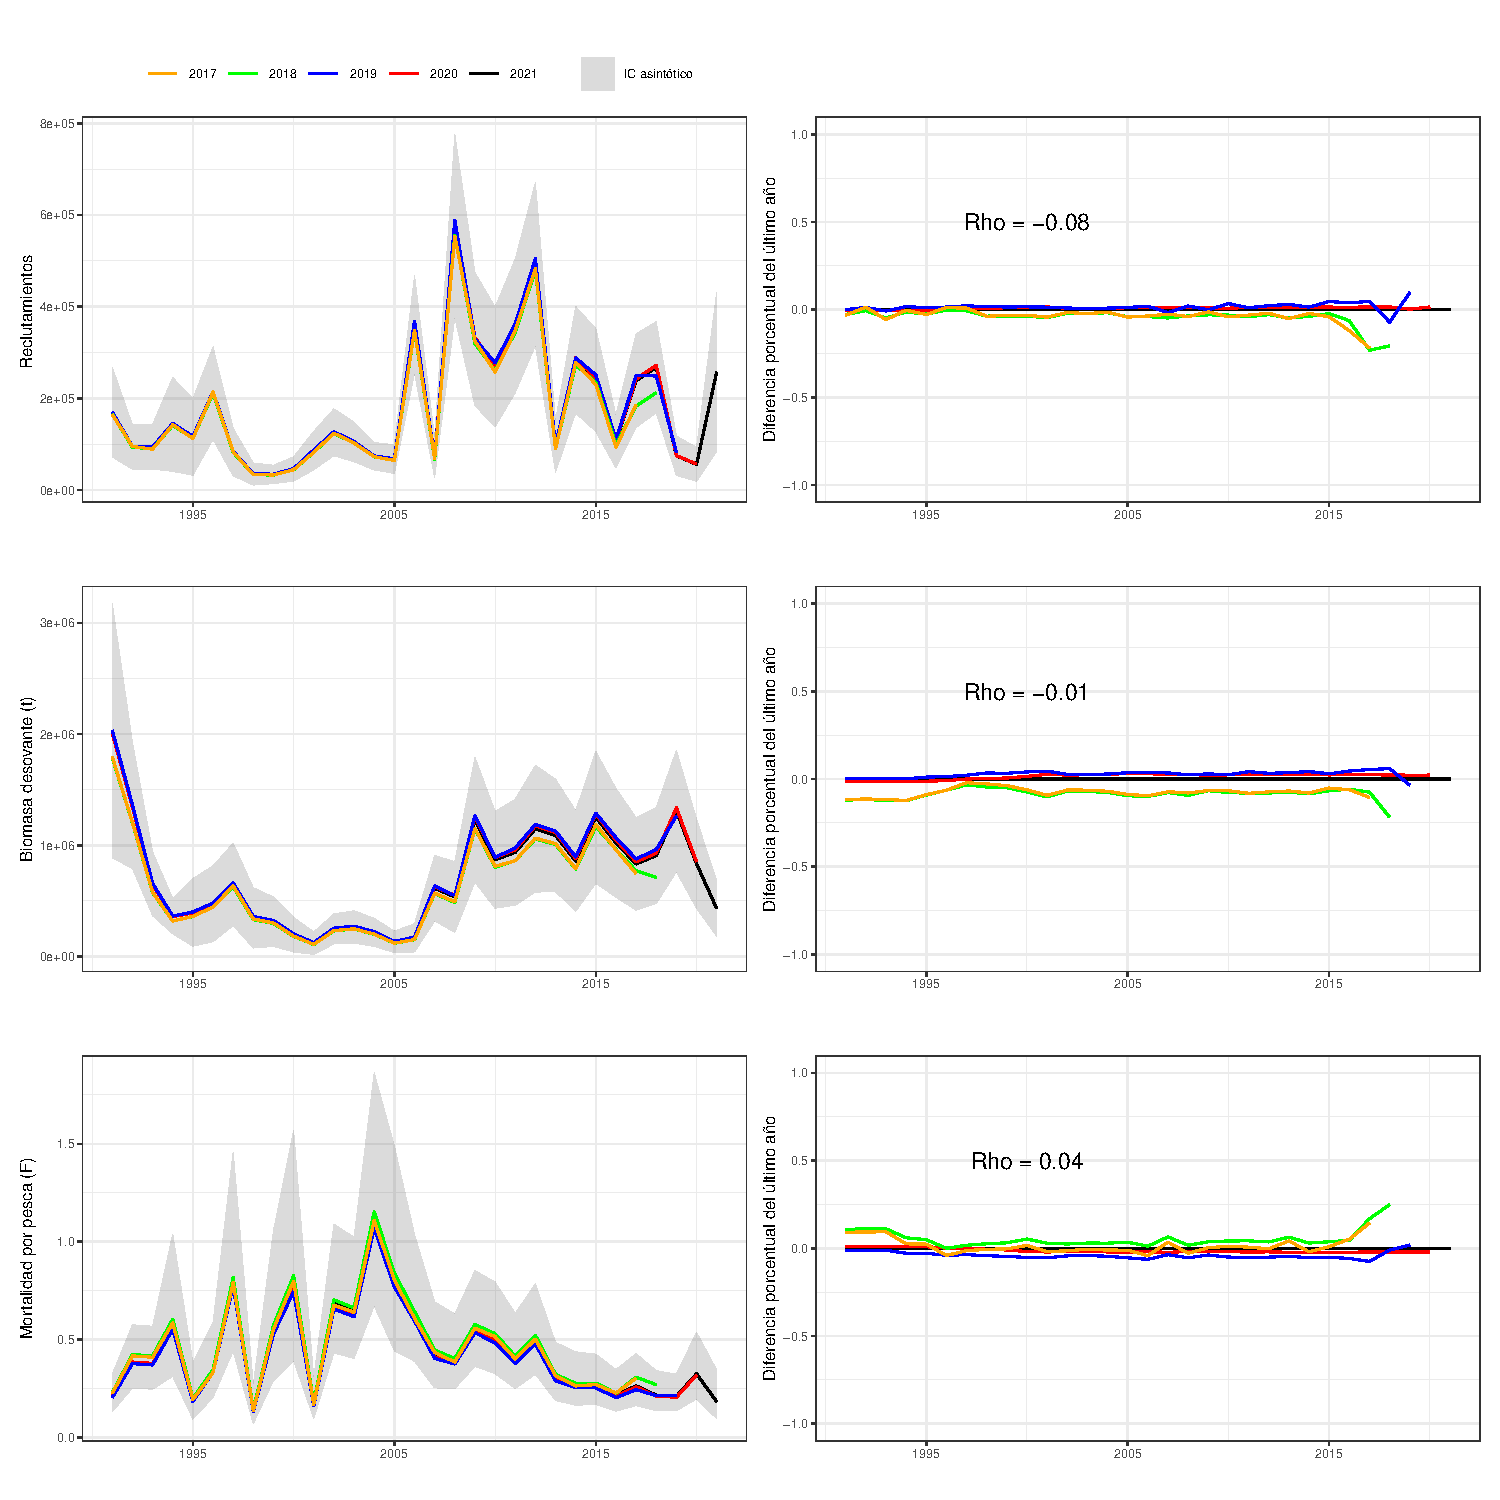
\includegraphics[width=0.7\textwidth]{FigurasInforme_Marzo/F33_retrospectivo_marzo-1.pdf}
\end{center}
\end{frame}

\begin{frame}{Comparación con asesorías previas de sardina común}
\protect\hypertarget{comparaciuxf3n-con-asesoruxedas-previas-de-sardina-comuxfan}{}
\begin{center}
\includegraphics[width=0.7\textwidth]{FigurasInforme_Marzo/F32_comparación_marzo-1.pdf}
\end{center}
\end{frame}

\end{document}
